\section{Metodologia}
\label{sec:metodologia}

A contribuição para a comunidade do Noosfero, no contexto do Comunidade.UnB e
do Portal da UnB Gama, é realizada por uma equipe de estagiários do LAPPIS,
assim como pela equipe do projeto do Novo Portal do Software Público%
\footnote{\url{http://www.participa.br/softwarepublico/}}, um projeto da UnB
em parceria com o Ministério do Planejamento, Orçamento e Gestão (MP). Nesta
seção apresentamos algumas práticas e metodologias utilizadas na evolução da
ferramenta. Na seção \ref{sec:resultados} apresentaremos
algumas funcionalidades desenvolvidas por nós de forma a adaptar o Noosfero
para o ambiente de uma universidade.

O processo de colaboração com o Noosfero inclui uma série de práticas apresentadas
pelas metodologias ágeis de desenvolvimento de software como o uso de testes
automatizados, a descrição das funcionalidades do projeto no formato de
histórias de usuário e a adoção de ferramentas para a utilização da metodologia
\textit{Behavior Driven Development} (BDD)%
\footnote{\url{http://en.wikipedia.org/wiki/Behavior-driven_development}},
uma evolução do \textit{Test Driven Development} (TDD)%
\footnote{\url{http://en.wikipedia.org/wiki/Test-driven_development}}
apresentada por Dan North \cite{north2006}.
%
As semelhanças das práticas adotadas pelas comunidades de software livre e as
comunidades de métodos ágeis foram apresentadas por Corbucci
em sua dissertação de mestrado \cite{corbucci2011}. De acordo com ele, os dois
métodos possuem tantas características em comum ao ponto de, Martin Fowler,
um dos autores mais influentes na Literatura sobre métodos ágeis,
incluir software livre como um método ágil na primeira versão de seu artigo
\textit{"The New Methodology"}. No entanto, o mesmo foi retirado devido
à falta de descrição precisa dos métodos de desenvolvimento utilizados pelas
comunidades de software livre \cite{fowler2000}.

Por outro lado, Corbuccy discute os princípios ágeis e livres
como semelhantes \cite{corbucci2011} :
%
(\textit{i}) Indivíduos e interações são mais importantes que processos e
ferramentas;
(\textit{ii}) Software em funcionamento é mais importante que documentação
abrangente;
(\textit{iii}) Colaboração com o cliente (usuários) é mais importante que
negociação de contratos;
(\textit{iv}) Responder às mudanças é mais importante que seguir um plano.
%
Também, explicita as práticas disseminadas pelas metodologias ágeis usadas no
cotidiano dos desenvolvedores de software livre:
(\textit{i}) Código compartilhado (coletivo);
(\textit{ii}) Projeto simples;
(\textit{iii}) Repositório único de código;
(\textit{iv}) Integração contínua;
(\textit{v}) Código e teste;
(\textit{vi}) Desenvolvimento dirigido por testes, e
(\textit{vii}) Refatoração~\cite{corbucci2011}. Portanto, neste trabalho,
entendemos software livre como um método ágil de desenvolvimento, do ponto de
vista da Engenharia de Software.

\begin{figure}[htpb]
    \begin{center}
        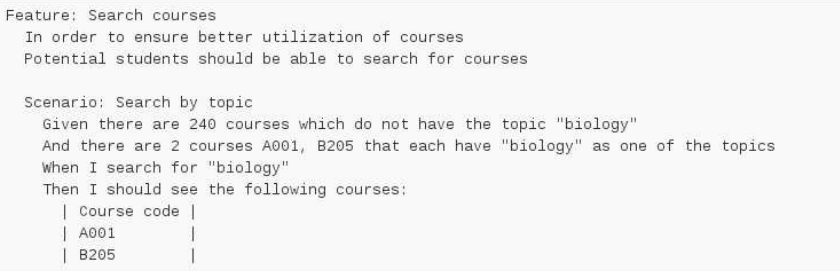
\includegraphics[width=.37\textwidth]{images/cucumber-sample.png}
    \end{center}
    \caption{Exemplo dee utilização do cucumber}
    \label{cucumber}
\end{figure}

Para especificarmos as funcionalidades desenvolvidas por nós, utilizamos
o formato de Histórias de Usuários (\textit{User Stories}),
prática bastante difundida dentro das comunidades de métodos ágeis e também
adotada em algumas comunidades de software livre.
%
Além das histórias, utilizamos também o formato de critérios de aceitação
apresentados por Dan North \cite{north2006}, outra
prática ágil que vem ganhando força com a popularização do BDD.
%
O formato adotado é conveniente para nós, uma vez que o Noosfero utiliza o
\textit{cucumber}\footnote{\url{http://cukes.info/}}, uma ferramenta para
automatização de testes escritos em linguagem natural, criada para apoiar a
utilização de BDD. No \textit{cucumber}, os testes são escritos no formato
de funcionalidades e cenários, utilizando os formatos de histórias de
usuário e de critérios de aceitação mencionados. A Figura
\ref{cucumber}\footnote{Extraído de \url{https://github.com/cucumber/cucumber/wiki}}
apresenta um exemplo de uso do \textit{cucumber}.

O processo de desenvolvimento de software utilizado durante este trabalho
também se baseia em metodologias ágeis, com a utilização de ciclos curtos de
forma a permitir que haja \textit{feedback} de forma mais rápida e reuniões
curtas periodicamente na qual os integrantes da equipe apresentam o andamento
das funcionalidades previstas para aquele ciclo e os impedimentos encontrados.
